\documentclass[aspectratio=169]{beamer}

% Theme
\usetheme{Madrid}
\usecolortheme{whale}

% Packages
\usepackage[utf8]{inputenc}
\usepackage{tikz}
\usepackage{listings}
\usepackage{booktabs}

% TikZ libraries
\usetikzlibrary{shapes, arrows, positioning}

% Colors
\definecolor{primaryblue}{RGB}{0, 102, 204}
\definecolor{successgreen}{RGB}{40, 167, 69}
\definecolor{dangerred}{RGB}{220, 53, 69}
\definecolor{codebg}{RGB}{245, 245, 245}

% Listings
\lstset{
    basicstyle=\ttfamily\small,
    backgroundcolor=\color{codebg},
    frame=single,
    breaklines=true
}

% Title
\title[Git \& GitHub]{Version Control: Git and GitHub}
\subtitle{CS2113 -- Software Development Project}
\author{Masoud Hamad}
\institute{School of Computing Communication and Media Studies}
\date{Academic Year 2025}

\begin{document}

%============================================================
\begin{frame}
    \titlepage
\end{frame}

%============================================================
\begin{frame}{Outline}
    \tableofcontents
\end{frame}

%============================================================
\section{Introduction to Version Control}
%============================================================

\begin{frame}{What is Version Control?}
    \begin{block}{Definition}
        A system for storing code that enables tracking, sharing, and managing changes.
    \end{block}

    \vspace{0.3cm}

    \textbf{Benefits:}
    \begin{itemize}
        \item Store backups of current and older versions
        \item Enable collaboration without meeting in person
        \item Track who made what changes
        \item Recover previous project states
        \item Identify when bugs were introduced
    \end{itemize}
\end{frame}

%============================================================
\begin{frame}{Git and GitHub}
    \begin{columns}
        \begin{column}{0.5\textwidth}
            \textbf{Git}
            \begin{itemize}
                \item Created by Linus Torvalds
                \item Distributed version control
                \item Runs locally on your machine
                \item Free and open source
            \end{itemize}
        \end{column}
        \begin{column}{0.5\textwidth}
            \textbf{GitHub}
            \begin{itemize}
                \item Cloud hosting for Git repos
                \item Collaboration features
                \item Issues, PRs, Projects
                \item Industry standard
            \end{itemize}
        \end{column}
    \end{columns}
\end{frame}

%============================================================
\section{Git Basics}
%============================================================

\begin{frame}[fragile]{Initial Setup}
    \begin{lstlisting}[language=bash]
# Configure your identity
git config --global user.name "Your Name"
git config --global user.email "email@example.com"
git config --global init.defaultBranch main
    \end{lstlisting}

    \begin{alertblock}{Important}
        Use the same email as your GitHub account!
    \end{alertblock}
\end{frame}

%============================================================
\begin{frame}[fragile]{Starting a Project}
    \begin{lstlisting}[language=bash]
# Initialize a new Git repository
git init

# Check status
git status
    \end{lstlisting}

    \begin{block}{What happens?}
        Creates a \texttt{.git} folder storing all project metadata and history.
    \end{block}
\end{frame}

%============================================================
\begin{frame}{Understanding Commits}
    \begin{center}
    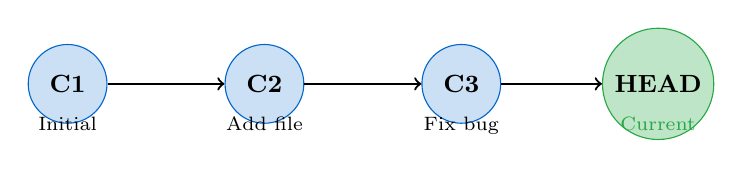
\begin{tikzpicture}[
        commit/.style={circle, draw=primaryblue, fill=primaryblue!20, minimum size=1cm, font=\small\bfseries}
    ]
        \node[commit] (c1) at (0, 0) {C1};
        \node[commit] (c2) at (2.5, 0) {C2};
        \node[commit] (c3) at (5, 0) {C3};
        \node[commit, fill=successgreen!30, draw=successgreen] (head) at (7.5, 0) {HEAD};

        \draw[->, thick] (c1) -- (c2);
        \draw[->, thick] (c2) -- (c3);
        \draw[->, thick] (c3) -- (head);

        \node[below=0.3cm, font=\scriptsize] at (c1) {Initial};
        \node[below=0.3cm, font=\scriptsize] at (c2) {Add file};
        \node[below=0.3cm, font=\scriptsize] at (c3) {Fix bug};
        \node[below=0.3cm, font=\scriptsize, successgreen] at (head) {Current};
    \end{tikzpicture}
    \end{center}

    \begin{block}{A Commit is...}
        A bundle of changes -- a snapshot of your project at a point in time.
    \end{block}
\end{frame}

%============================================================
\begin{frame}{File States in Git}
    \begin{center}
    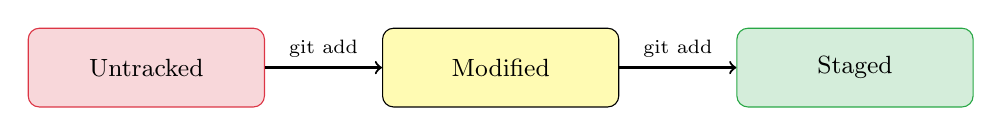
\begin{tikzpicture}[
        state/.style={rectangle, draw, rounded corners, minimum width=3cm, minimum height=1cm, align=center, font=\small}
    ]
        \node[state, fill=dangerred!20, draw=dangerred] (untracked) at (0, 0) {Untracked};
        \node[state, fill=yellow!30] (modified) at (4.5, 0) {Modified};
        \node[state, fill=successgreen!20, draw=successgreen] (staged) at (9, 0) {Staged};

        \draw[->, thick] (untracked) -- node[above, font=\scriptsize] {git add} (modified);
        \draw[->, thick] (modified) -- node[above, font=\scriptsize] {git add} (staged);
    \end{tikzpicture}
    \end{center}

    \vspace{0.5cm}

    \begin{itemize}
        \item \textcolor{dangerred}{\textbf{Untracked:}} New files unknown to Git
        \item \textcolor{yellow!80!black}{\textbf{Modified:}} Changed but not staged
        \item \textcolor{successgreen}{\textbf{Staged:}} Ready for commit
    \end{itemize}
\end{frame}

%============================================================
\begin{frame}[fragile]{The Commit Workflow}
    \begin{lstlisting}[language=bash]
# 1. Make changes to files

# 2. Stage changes
git add filename.txt
git add .  # Add all changes

# 3. Create commit
git commit -m "Descriptive message"

# 4. Check status
git status
    \end{lstlisting}
\end{frame}

%============================================================
\section{Working with GitHub}
%============================================================

\begin{frame}{Local vs Remote Repository}
    \begin{center}
    
\begin{tikzpicture}[
        repo/.style={rectangle, draw, rounded corners, minimum width=3.5cm, minimum height=1.5cm, align=center}
    ]
        \node[repo, fill=primaryblue!20, draw=primaryblue] (local) at (0, 0) {\textbf{Local}\\Your Computer};
        \node[repo, fill=successgreen!20, draw=successgreen] (remote) at (7, 0) {\textbf{Remote}\\GitHub};

        \draw[->, thick, primaryblue] ([yshift=0.3cm]local.east) -- node[above, font=\small] {git push} ([yshift=0.3cm]remote.west);
        \draw[->, thick, successgreen] ([yshift=-0.3cm]remote.west) -- node[below, font=\small] {git pull} ([yshift=-0.3cm]local.east);
    \end{tikzpicture}
    \end{center}
\end{frame}

%============================================================
\begin{frame}[fragile]{Connecting to GitHub}
    \begin{lstlisting}[language=bash]
# Add remote repository
git remote add origin https://github.com/user/repo.git

# Push to remote (first time)
git push -u origin main

# Push subsequent changes
git push

# Pull changes from remote
git pull
    \end{lstlisting}
\end{frame}

%============================================================
\begin{frame}[fragile]{Cloning a Repository}
    \begin{lstlisting}[language=bash]
# Clone existing repository
git clone https://github.com/user/repo.git

# Clone into specific folder
git clone https://github.com/user/repo.git folder-name
    \end{lstlisting}

    \begin{alertblock}{Note}
        To push to a cloned repo, you need collaborator access!
    \end{alertblock}
\end{frame}

%============================================================
\section{Branches}
%============================================================

\begin{frame}{Understanding Branches}
    \begin{center}
    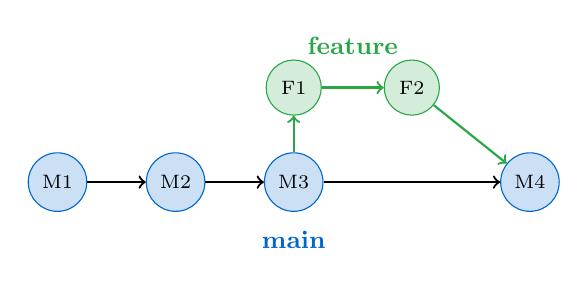
\begin{tikzpicture}[
        commit/.style={circle, draw=primaryblue, fill=primaryblue!20, minimum size=0.7cm, font=\scriptsize},
        feature/.style={circle, draw=successgreen, fill=successgreen!20, minimum size=0.7cm, font=\scriptsize}
    ]
        \node[commit] (m1) at (0, 0) {M1};
        \node[commit] (m2) at (1.5, 0) {M2};
        \node[commit] (m3) at (3, 0) {M3};
        \node[commit] (m4) at (6, 0) {M4};

        \node[feature] (f1) at (3, 1.2) {F1};
        \node[feature] (f2) at (4.5, 1.2) {F2};

        \draw[->, thick] (m1) -- (m2);
        \draw[->, thick] (m2) -- (m3);
        \draw[->, thick, successgreen] (m3) -- (f1);
        \draw[->, thick, successgreen] (f1) -- (f2);
        \draw[->, thick, successgreen] (f2) -- (m4);
        \draw[->, thick] (m3) -- (m4);

        \node[below, primaryblue, font=\small\bfseries] at (3, -0.5) {main};
        \node[above, successgreen, font=\small\bfseries] at (3.75, 1.5) {feature};
    \end{tikzpicture}
    \end{center}

    \begin{block}{Purpose}
        Branches allow parallel development without affecting the main code.
    \end{block}
\end{frame}

%============================================================
\begin{frame}[fragile]{Branch Commands}
    \begin{lstlisting}[language=bash]
# Create new branch
git branch feature-name

# Switch to branch
git checkout feature-name

# Create and switch (shortcut)
git checkout -b feature-name

# List all branches
git branch

# Merge branch into current
git merge feature-name
    \end{lstlisting}
\end{frame}

%============================================================
\section{Handling Conflicts}
%============================================================

\begin{frame}[fragile]{Merge Conflicts}
    When two people change the same lines:

    \begin{lstlisting}
<<<<<<< HEAD
Your local changes
=======
Changes from remote
>>>>>>> abc123def
    \end{lstlisting}

    \textbf{Resolution:}
    \begin{enumerate}
        \item Edit file -- choose/combine changes
        \item Remove conflict markers
        \item \texttt{git add filename}
        \item \texttt{git commit}
    \end{enumerate}
\end{frame}

%============================================================
\section{Best Practices}
%============================================================

\begin{frame}{Git Best Practices}
    \begin{enumerate}
        \item \textbf{Pull before starting} any development
        \item Make \textbf{small, focused commits} with clear messages
        \item \textbf{Push frequently} to backup your work
        \item Use \textbf{branches} for new features
        \item \textbf{Never commit sensitive data} (passwords, keys)
        \item \textbf{Communicate} with team about file ownership
    \end{enumerate}

    \begin{alertblock}{Warning}
        Once pushed, secrets are in history forever!
    \end{alertblock}
\end{frame}

%============================================================
\begin{frame}{Command Reference}
    \begin{center}
    \begin{tabular}{ll}
        \toprule
        \textbf{Command} & \textbf{Description} \\
        \midrule
        \texttt{git init} & Initialize repository \\
        \texttt{git clone <url>} & Clone remote repo \\
        \texttt{git status} & Check current status \\
        \texttt{git add <file>} & Stage changes \\
        \texttt{git commit -m "msg"} & Create commit \\
        \texttt{git push} & Push to remote \\
        \texttt{git pull} & Pull from remote \\
        \texttt{git log} & View history \\
        \bottomrule
    \end{tabular}
    \end{center}
\end{frame}

%============================================================
\begin{frame}{Questions?}
    \begin{center}
        \Huge Questions?
    \end{center}
\end{frame}

\end{document}
